\documentclass[11pt,a4paper]{article}

\usepackage[utf8]{inputenc}
\usepackage[T1]{fontenc}
\usepackage[spanish,es-tabla]{babel}
\usepackage{lmodern}
\usepackage[margin=2.5cm]{geometry}
\usepackage{graphicx}
\usepackage{booktabs}
\usepackage{float}
\usepackage{caption}
\usepackage{listings}
\usepackage{xcolor}
\usepackage{tikz}
\usetikzlibrary{positioning,arrows.meta}
\usepackage[hidelinks]{hyperref}

\lstset{
  basicstyle=\ttfamily\small,
  columns=fullflexible,
  keepspaces=true,
  frame=single,
  framerule=0.3pt,
  rulecolor=\color{gray!60},
  backgroundcolor=\color{gray!6},
  breaklines=true,
  showstringspaces=false,
  literate={á}{{\'a}}1 {é}{{\'e}}1 {í}{{\'i}}1 {ó}{{\'o}}1 {ú}{{\'u}}1 {ñ}{{\~n}}1
}

\setlength{\parskip}{0.5em}
\setlength{\parindent}{0pt}

\begin{document}

\begin{titlepage}
  \centering
  {\large Universidad de Ingeniería y Tecnología (UTEC)\par}
  {\large Escuela de Ciencia de la Computación\par}
  \vspace{0.5cm}
  {\large Curso: Base de Datos 2, ciclo 2026-2\par}
  \vspace{3cm}
  {\LARGE Minigestor de base de datos multimodal\par}
  \vspace{0.5cm}
  {\Large Informe del proyecto: Parte 1 (base de datos relacional) y Parte 2 (base de datos espacial)\par}
  \vspace{3cm}
  {\large Integrantes\par}
  \vspace{0.3cm}
  Luis Izaguirre\par
  Dayane Rojas\par
  Noe Paredes\par
  Jimena Huamani\par
  Omar Chavarria\par
  \vfill
  {\large Lima, 4 de octubre de 2026\par}
  \vspace{0.3cm}
  Repositorio: \url{https://github.com/LuisIZ/BD2_Proyecto_2026-2}\par
\end{titlepage}

\tableofcontents
\newpage

%-------------------------------------------------------------------------------
\section{Introducción}

El proyecto consiste en construir desde cero un gestor de bases de datos que soporte varios tipos de datos. Este informe cubre las dos primeras partes del enunciado. La Parte 1 corresponde a una base de datos relacional con tablas y SQL: organización de archivos en disco, índices, algoritmos externos, procesamiento de consultas, transacciones y una interfaz gráfica. La Parte 2 extiende el motor con datos espaciales: coordenadas geográficas, métricas de distancia y consultas por radio y por cercanía.

El objetivo del curso no es competir con un motor comercial, sino entender cómo funciona por dentro. Por eso el equipo escribió cada estructura sobre páginas de 4 KB y midió cuántas páginas lee y escribe cada operación. Esa medida, más que el tiempo, es la que permite explicar por qué una técnica conviene más que otra.

El informe sigue la estructura pedida en la sección de entregables: primero la arquitectura y el dominio de datos, luego la explicación de cada técnica implementada y al final la comparación experimental. La última sección resume lo que quedó pendiente. El código fuente, la documentación técnica de cada módulo y este informe están en el repositorio del proyecto: \url{https://github.com/LuisIZ/BD2_Proyecto_2026-2}.

%-------------------------------------------------------------------------------
\section{Arquitectura del sistema}

El sistema está dividido en capas. Cada capa solo conoce a la que tiene debajo, lo que permitió que distintos integrantes trabajaran en paralelo sobre interfaces acordadas.

\begin{figure}[H]
\centering
\begin{tikzpicture}[
  capa/.style={draw, rounded corners=2pt, minimum width=11cm, minimum height=0.9cm, align=center, fill=gray!8},
  flecha/.style={-{Stealth[length=2mm]}, thick}]
\node[capa] (web) {Interfaz web (React + TypeScript): archivos, consultas, resultados, plan y comparación};
\node[capa, below=0.35cm of web] (api) {API (Python + FastAPI): recibe el SQL y llama al binario \texttt{motor\_sql}};
\node[capa, below=0.35cm of api] (sql) {Consultas (C++): parser, planificador, ejecutor, EXPLAIN, transacciones};
\node[capa, below=0.35cm of sql] (alg) {Algoritmos externos: merge sort k-way y external hashing};
\node[capa, below=0.35cm of alg] (idx) {Índices: B+ agrupado, B+ no agrupado, hash extensible y R-Tree en disco};
\node[capa, below=0.35cm of idx] (arc) {Archivos: Heap File con páginas slotted y archivo secuencial paginado};
\node[capa, below=0.35cm of arc] (pag) {Páginas de 4 KB en disco, gestor de páginas y buffer pool de 64 marcos};
\foreach \a/\b in {web/api, api/sql, sql/alg, alg/idx, idx/arc, arc/pag} \draw[flecha] (\a) -- (\b);
\end{tikzpicture}
\caption{Capas del minigestor.}
\end{figure}

El motor está escrito en C++17 y se compila con un \texttt{Makefile}. Su punto de entrada es el binario \texttt{motor\_sql}, que recibe un lote de sentencias SQL y responde en JSON con las filas, el plan de ejecución y las páginas leídas. La API en Python solo traduce peticiones HTTP a llamadas a ese binario, y la interfaz web dibuja las respuestas. Así, todo lo que toca el disco está en C++ y puede probarse sin la interfaz.

\subsection{Organización del código}

\begin{lstlisting}
motor/
  comun/          interfaz IFileOrganization y Registro, compartidos
  archivos/       heap_file, sequential_file, pagina_slotted
  indices/        bplus_agrupado, bplus_no_agrupado, hash_extensible_disco,
                  rtree, gestor_paginas, buffer_pool
  consultas/      parser_sql, catalogo, ejecutor, external_algorithms, motor_sql
  espacial/       distancia.h (métricas euclidiana y haversine)
  transacciones/  gestor_locks.h (2PL estricto y deadlocks)
  pruebas/        una prueba por estructura y los benchmarks
api/              API en Python que llama al motor
web/              interfaz React
datos/            datasets CSV y resultados de los experimentos
docs/             documentación técnica de cada módulo y este informe
\end{lstlisting}

Cada módulo tiene su prueba en \texttt{motor/pruebas/}, y \texttt{make test} las ejecuta todas. Al momento de entregar, los diez programas de prueba terminan sin errores.

%-------------------------------------------------------------------------------
\section{Dominio de datos}

\subsection{Datasets}

El conjunto principal es \texttt{organizations}, un CSV público con datos de empresas en tres tamaños: 1\,000, 10\,000 y 100\,000 filas. Sus columnas son \texttt{Index}, \texttt{Organization Id}, \texttt{Name}, \texttt{Website}, \texttt{Country}, \texttt{Description}, \texttt{Founded}, \texttt{Industry} y \texttt{Number of employees}. La columna \texttt{Index} es un entero único y sirve como clave primaria; \texttt{Founded} y \texttt{Number of employees} son enteros con muchos valores repetidos, útiles para probar índices secundarios. La fila promedio mide unos 140 bytes y la más larga 220 bytes.

Para la Parte 2 se usan puntos de Lima (centro, San Isidro, Miraflores, Barranco y Callao) en las pruebas de distancia, y un archivo pequeño de alumnos sirve para probar tablas creadas a mano.

\subsection{Tipos de datos}

El motor maneja tres tipos de columna:

\begin{itemize}
  \item \texttt{INT}: entero de 32 bits.
  \item \texttt{VARCHAR(n)}: texto de hasta $n$ bytes.
  \item \texttt{POINT}: coordenada geográfica (latitud, longitud). Se guarda como dos enteros de 32 bits en microgrados, es decir, grados multiplicados por un millón. Ocupa 8 bytes y tiene una precisión de unos 11 cm.
\end{itemize}

La clave primaria debe ser \texttt{INT} y puede estar en cualquier columna. Los decimales de las coordenadas se convierten a microgrados leyendo las cifras como texto, sin pasar por números de punto flotante, para que \texttt{POINT(-12.0464, -77.0428)} se guarde exactamente como \texttt{-12046400} y \texttt{-77042800}.

\subsection{Formato de registro y de página}

Todas las estructuras trabajan sobre páginas de 4\,096 bytes. En el Heap File y en el archivo secuencial, un registro es \texttt{[int32 clave][uint32 largo][valor]}, donde el valor empaqueta el resto de columnas: los enteros en 4 bytes y los textos con su largo en 2 bytes seguido de los caracteres. El B+ agrupado usa registros de tamaño fijo, con la clave primero y cada texto rellenado hasta su largo máximo, para poder ubicarlos por posición dentro de la hoja.

%-------------------------------------------------------------------------------
\section{Parte 1: técnicas implementadas}

\subsection{Heap File con páginas slotted}

El Heap File guarda los registros en orden de llegada. Cada página tiene una cabecera con el número de slots y el inicio del espacio libre, un directorio de slots que crece hacia abajo y los datos que crecen desde el final hacia arriba. Un registro se identifica por su RID, el par (página, slot), y ese RID no cambia aunque otros registros se borren, porque borrar solo marca el slot como tumba.

Para reutilizar espacio, el archivo mantiene en memoria un mapa del espacio libre de cada página, que se reconstruye al abrir leyendo solo las cabeceras. Así una inserción no recorre el archivo buscando sitio: consulta el mapa, lee una página y la escribe. La prueba del enunciado (insertar 1\,000, borrar 500 e insertar 500) termina sin que el archivo crezca.

La desventaja es que el heap no tiene orden, así que buscar por clave primaria sin índice obliga a recorrer el archivo.

\subsection{Archivo secuencial paginado}

El archivo secuencial mantiene los registros ordenados por clave dentro de cada página y entre páginas. Tiene un área principal ordenada y un área auxiliar donde van los registros que no caben en su página.

\begin{itemize}
  \item La búsqueda hace búsqueda binaria sobre las páginas principales leyendo solo la primera clave de cada una, luego búsqueda binaria dentro de la página y, si no encuentra la clave, recorre el auxiliar.
  \item La inserción ubica la página por búsqueda binaria; si hay espacio, inserta en su posición ordenada, y si no, el registro va al área auxiliar.
  \item La eliminación es perezosa: marca el slot como tumba y lo deja en su sitio, porque su clave todavía sirve como frontera para la búsqueda binaria.
  \item La reorganización se dispara cuando las tumbas y los registros auxiliares superan el 30\,\% del total. Hace una mezcla en streaming del área principal con el auxiliar ordenado y deja las páginas al 80\,\% para que las siguientes inserciones entren en su lugar.
\end{itemize}

\subsection{B+ agrupado}

En el B+ agrupado las hojas del árbol contienen las filas completas, ordenadas por clave primaria, y están encadenadas. Una búsqueda baja de la raíz a la hoja leyendo una página por nivel, y un rango recorre hojas consecutivas. Con filas de 180 bytes caben 22 registros por hoja. El árbol implementa split de hojas y nodos internos con propagación hasta la raíz, eliminación con préstamo y fusión, y una carga masiva que construye las hojas al 90\,\% de su capacidad. Solo puede haber uno por tabla, porque define el orden físico de los datos.

\subsection{B+ no agrupado}

El B+ no agrupado es un índice secundario: sus hojas guardan pares (clave, RID) que apuntan al Heap File, con 16 bytes por entrada y unas 205 entradas por página. Admite claves repetidas y puede crearse sobre cualquier columna \texttt{INT} con \texttt{CREATE INDEX}. Su costo está en que cada fila encontrada obliga a leer una página del heap, y esas páginas están dispersas.

\subsection{Hash extensible en disco}

El hash extensible mantiene un directorio de $2^d$ punteros a buckets, donde $d$ es la profundidad global. Cada bucket es una página de 4 KB con 255 entradas (clave, RID). Cuando un bucket se llena y sus entradas pueden separarse por un bit más del hash, se divide, y si su profundidad local ya era igual a la global, el directorio se duplica. Si todas las entradas tienen la misma clave, dividir no sirve, y en ese caso se encadena una página de desborde. La profundidad máxima es un parámetro del constructor y por defecto vale 16 bits (65\,536 entradas de directorio), un valor que el profesor sugirió revisar en el primer avance. Al llegar a ese límite el directorio deja de duplicarse y los buckets llenos pasan a usar páginas de desborde.

El hash responde una igualdad con una lectura del directorio y una del bucket, pero no tiene noción de orden, así que el planificador nunca lo usa para rangos.

\subsection{Algoritmos externos}

\paragraph{External merge sort.} Para \texttt{ORDER BY}, los registros se dividen en corridas del tamaño del presupuesto de memoria (páginas de buffer por registros por página). Cada corrida se ordena y luego se mezclan $k$ a la vez con un heap de mínimos, en $O(N \log k)$. La traza del plan reporta las corridas iniciales y las pasadas de mezcla.

\paragraph{External hashing para GROUP BY.} Las filas se reparten en particiones según el hash de la columna de agrupación. Como todas las filas de un grupo caen en la misma partición, cada partición se agrega por separado con su propia tabla de hash y luego se libera. Así en memoria solo viven los grupos de la partición en curso: con 300 grupos repartidos en 9 particiones, el máximo de grupos simultáneos fue 42. El plan muestra ese valor como \texttt{grupos\_en\_memoria}.

\subsection{Parser, planificador y EXPLAIN}

El parser es de descenso recursivo y reconoce \texttt{CREATE TABLE} (con esquema o desde un CSV), \texttt{COPY}, \texttt{CREATE INDEX ... USING BPLUS | HASH}, \texttt{INSERT}, \texttt{DELETE}, \texttt{SELECT} con \texttt{WHERE}, \texttt{GROUP BY}, \texttt{ORDER BY} y \texttt{LIMIT}, \texttt{DROP}, \texttt{SHOW TABLES}, \texttt{DESCRIBE}, \texttt{EXPLAIN [ANALYZE]} y las sentencias de transacción.

El planificador elige una sola condición del \texttt{WHERE} que pueda resolverse con una estructura (índice, clave del agrupado o búsqueda binaria del secuencial) y deja el resto para un filtro en memoria. La decisión se toma mirando solo el catálogo, sin leer datos, y por eso \texttt{EXPLAIN} puede mostrar el plan sin ejecutar la consulta. \texttt{EXPLAIN ANALYZE} sí la ejecuta y agrega a cada nodo las filas, páginas y milisegundos reales, y termina con el tiempo de planificación (que incluye el parseo) y el de ejecución, como en PostgreSQL:

\begin{lstlisting}
Limit on t  (rows=3) (actual rows=3)
  -> Projection on t (actual rows=15)
    -> Sort on t (actual time=1.151 rows=15)
       Sort Key: Index ASC
      -> Index Scan using idx_f on t (Founded)  (cost=4.00 rows=1) (actual time=0.187 rows=15 pages=17)
         Index Cond: Founded = 2005
Rows: 3
Planning Time: 1.131 ms
Execution Time: 2.400 ms
\end{lstlisting}

El costo se expresa en páginas estimadas. Para un índice no agrupado cuenta la altura del árbol más una página de datos por fila, que es justamente lo que lo vuelve caro en rangos anchos.

\subsection{Transacciones y concurrencia}

El motor reconoce \texttt{BEGIN TRANSACTION}, \texttt{END TRANSACTION} (o \texttt{COMMIT}) y \texttt{ROLLBACK}. El control de concurrencia usa locks a nivel de tabla: un \texttt{SELECT} pide un lock compartido (S) y un \texttt{INSERT} o \texttt{DELETE} pide uno exclusivo (X). Se aplica 2PL estricto, es decir, los locks de una transacción se conservan hasta que termina, y la espera se implementa con variables de condición, sin espera activa.

Para los deadlocks se optó por detección. Cuando una transacción debe esperar, el gestor arma el grafo de espera y busca un ciclo con una búsqueda en profundidad. Si lo encuentra, aborta a la transacción más joven del ciclo y registra el ciclo y el motivo. Como las páginas se escriben en disco en el momento, el rollback es un deshacer lógico: cada \texttt{INSERT} y \texttt{DELETE} de la transacción queda anotado y \texttt{ROLLBACK} aplica la operación inversa en orden contrario.

La demostración con hilos se describe en la sección \ref{sec:demo}.

\subsection{Interfaz de usuario}

La interfaz web tiene los cuatro paneles pedidos: archivos (tablas, esquema, índices y estadísticas de páginas), consultas (editor con resaltado de SQL), resultados (tabla con contador y tiempo) y plan de ejecución, que dibuja el árbol de operadores como grafo con las filas, el tiempo y el índice usado en cada nodo. Además incluye la carga de CSV con elección de clave primaria e índices, y una sección de comparación que ejecuta la misma consulta sobre las distintas organizaciones y grafica el resultado.

%-------------------------------------------------------------------------------
\section{Parte 2: base de datos espacial}

\subsection{Métricas de distancia}

El módulo \texttt{motor/espacial/distancia.h} implementa las dos métricas pedidas y devuelve metros:

\begin{itemize}
  \item Haversine (geodésica), la distancia sobre una esfera de 6\,371 km de radio. Es la que se usa por defecto.
  \item Euclidiana, la distancia en el plano de grados, convertida a metros con el mismo radio.
\end{itemize}

\begin{table}[H]
\centering
\begin{tabular}{lrr}
\toprule
Caso & Haversine & Euclidiana \\
\midrule
1° de latitud, o 1° de longitud sobre el ecuador & 111\,194.9 m & 111\,194.9 m \\
Lima centro a San Isidro & 5\,745.3 m & 5\,747.2 m \\
Lima a Cusco & 574.6 km & 588.0 km \\
1° de longitud a latitud 60° & 55\,596.9 m & 111\,194.9 m \\
\bottomrule
\end{tabular}
\caption{Distancias verificadas por \texttt{distancia\_test}.}
\end{table}

La última fila muestra el límite de la métrica euclidiana: trata un grado de longitud como si midiera lo mismo en cualquier latitud, cuando a 60° mide la mitad. Cerca del ecuador, como en Lima, las dos casi coinciden.

\subsection{Extensión SQL}

El parser se extendió con el tipo \texttt{POINT}, el literal \texttt{POINT(lat, lon)} y la función \texttt{distancia}:

\begin{lstlisting}[language=SQL]
CREATE TABLE tiendas (id INT PRIMARY KEY, nombre VARCHAR(20), ubicacion POINT);
INSERT INTO tiendas VALUES (1, 'Centro', POINT(-12.0464, -77.0428));
SELECT * FROM tiendas WHERE distancia(ubicacion, POINT(-12.0464, -77.0428)) < 5000;
SELECT * FROM tiendas ORDER BY distancia(ubicacion, POINT(-12.0464, -77.0428)) LIMIT 10;
\end{lstlisting}

Sin índice, la consulta por radio se resuelve como un filtro sobre la distancia y la de k vecinos ordena por distancia con el mismo merge sort externo del \texttt{ORDER BY}, cortando con \texttt{LIMIT}. Con un índice R-Tree, ambas se resuelven con el índice, como se explica en la siguiente subsección. Antes de ejecutar se valida que \texttt{distancia} reciba una columna \texttt{POINT} y que una columna \texttt{POINT} no se compare con \texttt{=} o \texttt{<}. Con cinco puntos de Lima, la consulta de los tres más cercanos al centro devuelve centro, San Isidro y Callao, y la de radio de 6 km devuelve centro y San Isidro, en las tres organizaciones de archivo.

\subsection{Índice R-Tree}

El R-Tree guarda los puntos en nodos de 4 KB, igual que los demás índices, con 170 entradas por nodo. Cada entrada tiene un rectángulo mínimo envolvente (MBR) en microgrados y una referencia: en una hoja es la posición del registro y en un nodo interno es la página del hijo. Para insertar se baja por la entrada cuyo MBR crece menos, y cuando un nodo se llena se divide con el split cuadrático de Guttman, que elige como semillas las dos entradas que más área desperdiciarían juntas y reparte el resto según cuánto crece cada grupo.

Las consultas usan las métricas del módulo de distancias:

\begin{itemize}
  \item Rango por radio: se calcula la caja de grados que contiene al círculo y solo se baja por los nodos cuyo MBR la corta; en las hojas se filtra con la distancia exacta.
  \item k vecinos: búsqueda \emph{best-first} con una cola de prioridad ordenada por la distancia mínima del punto a cada MBR. Como esa distancia nunca supera la de un punto dentro del rectángulo, los puntos salen de la cola ya ordenados del más cercano al más lejano.
\end{itemize}

Desde SQL, \texttt{CREATE INDEX idx\_geo ON tiendas (ubicacion) USING RTREE} construye el índice sobre una columna \texttt{POINT} de una tabla \texttt{HEAP} y el motor lo mantiene en cada \texttt{INSERT} y \texttt{DELETE}. El planificador lo usa para \texttt{distancia(...) < r} y para \texttt{ORDER BY distancia(...) LIMIT k}, y el plan lo muestra así:

\begin{lstlisting}
-> Index Scan using idx_geo on tiendas (ubicacion)  (cost=4.00 rows=1) (actual time=0.041 rows=2 pages=3)
   Index Cond: distancia(ubicacion, POINT(-12.046400, -77.042800)) [haversine] < 6000
\end{lstlisting}

\subsection{Intersección con polígono}

La tercera consulta del enunciado, puntos dentro de un polígono, se escribe así:

\begin{lstlisting}[language=SQL]
SELECT nombre FROM tiendas
WHERE dentro(ubicacion, POLYGON((-12.13 -77.05, -12.13 -77.02, -12.09 -77.02, -12.09 -77.05)));
\end{lstlisting}

La pertenencia se decide con \emph{ray casting}: desde el punto se traza un rayo y se cuentan los lados del polígono que cruza; si son impares, el punto está dentro. Las cuentas se hacen en microgrados con enteros de 64 bits, de modo que un punto sobre un borde se detecta de forma exacta y se considera dentro. Si la columna tiene R-Tree, el planificador pide al índice los puntos de la caja que envuelve al polígono y después aplica la prueba exacta solo a esos candidatos. En la prueba, un rectángulo alrededor de San Isidro y Miraflores devuelve esas dos tiendas, y un triángulo con la misma base devuelve solo Miraflores, con y sin índice.

\subsection{Estado de la Parte 2}

Están terminados el tipo \texttt{POINT}, las dos métricas, la extensión SQL, el índice R-Tree conectado al planificador, las consultas por radio, k vecinos y polígono, y la comparación experimental con GiST. La interfaz incluye además un panel de mapa con Leaflet que dibuja los puntos de la tabla sobre OpenStreetMap, resalta las filas que devolvió la consulta y traza el círculo de búsqueda o el polígono usado en el \texttt{WHERE}. Los límites se detallan en la sección \ref{sec:pendiente}.

%-------------------------------------------------------------------------------
\section{Comparación experimental}

\subsection{Metodología}

Todas las mediciones se hicieron en la misma máquina, con el dataset \texttt{organizations} de 1\,000, 10\,000 y 100\,000 filas y la semilla 42. Se reportan dos medidas: el tiempo de reloj y las páginas leídas o escritas, contadas por el propio motor. Los tiempos incluyen el caché de archivos del sistema operativo, así que reflejan CPU y llamadas al sistema más que la latencia de un disco real. Por eso las páginas son la medida más estable para comparar estructuras.

\subsection{Heap File frente a archivo secuencial}

\begin{table}[H]
\centering
\small
\begin{tabular}{lrrrrrr}
\toprule
& \multicolumn{3}{c}{Heap File} & \multicolumn{3}{c}{Secuencial} \\
\cmidrule(lr){2-4}\cmidrule(lr){5-7}
Operación & 1k & 10k & 100k & 1k & 10k & 100k \\
\midrule
Carga masiva (ms) & 1.7 & 16.1 & 111.4 & 8.0 & 15.0 & 117.9 \\
Inserción una a una (ms) & 20.7 & 167.0 & 1\,480.2 & 126.6 & 824.4 & 8\,330.9 \\
Búsqueda por clave (µs) & 89 & 877 & 11\,267 & 35 & 100 & 213 \\
Páginas por búsqueda & 16 & 158 & 1\,598 & 6 & 20 & 35 \\
Recorrido completo (ms) & 0.3 & 15.3 & 48.2 & 1.2 & 8.7 & 100.6 \\
Reorganización (ms) & 0.2 & 1.3 & 16.0 & 14.1 & 15.9 & 84.3 \\
Espacio en disco (MB) & 0.15 & 1.47 & 14.6 & 0.18 & 1.75 & 18.1 \\
\bottomrule
\end{tabular}
\caption{Heap File frente a archivo secuencial (medido el 4 de octubre de 2026).}
\end{table}

El heap inserta con una lectura y una escritura de página, y por eso es entre 5 y 6 veces más rápido al insertar fila por fila. El secuencial paga la búsqueda binaria de cada inserción, el área auxiliar y 20 reorganizaciones automáticas con 100\,000 filas. A cambio, el secuencial responde una búsqueda por clave leyendo 35 páginas en lugar de 1\,598, unas 50 veces menos.

Esta comparación explica la observación del primer avance sobre el tiempo del heap. El crecimiento no se debe a un error: sin índice, buscar por clave primaria en un heap es un recorrido, y su costo crece de forma lineal con el tamaño del archivo. El secuencial ocupa un 24\,\% más de disco porque sus páginas quedan al 80\,\% tras reorganizar. Con carga masiva, ambos tardan lo mismo, porque cada página se escribe una sola vez.

Una segunda medición, tomada como la mediana de 5 corridas (\nolinkurl{datos/resultados/heap_vs_secuencial.md}), confirma el mismo comportamiento: la búsqueda por clave en el heap pasa de 16 a 160 y a 1\,599 páginas al multiplicar los datos por 10, mientras que el secuencial pasa de 6 a 20 y a 35 páginas. Esa medición también muestra que el orden de llegada importa en el secuencial: con claves aleatorias el área auxiliar crece más (25\,629 registros con 100\,000 filas frente a 10\,625 con claves ascendentes) y la búsqueda lee 115 páginas en lugar de 35.

\subsection{Índices: B+ agrupado, B+ no agrupado y hash extensible}

Las seis gráficas siguientes comparan los tres índices sobre la misma clave y con registros de 180 bytes. Las mediciones del hash corresponden a la versión en memoria, que fue la usada en el primer avance. La comparación se repitió después con el hash ya en disco (\nolinkurl{datos/resultados/bplus_agrupado_vs_no_agrupado_vs_hash.md}, mediana de 5 corridas): contando la carga del heap, los tres índices se construyen en un tiempo parecido, entre 780 y 850 ms con 100\,000 filas, y la búsqueda por igualdad tarda 8,0 µs con el hash, 9,2 µs con el B+ agrupado y 11,0 µs con el B+ no agrupado. El hash en disco lee siempre 2 páginas de índice (directorio y bucket) y 1 del heap.

\begin{figure}[!htbp]
\centering
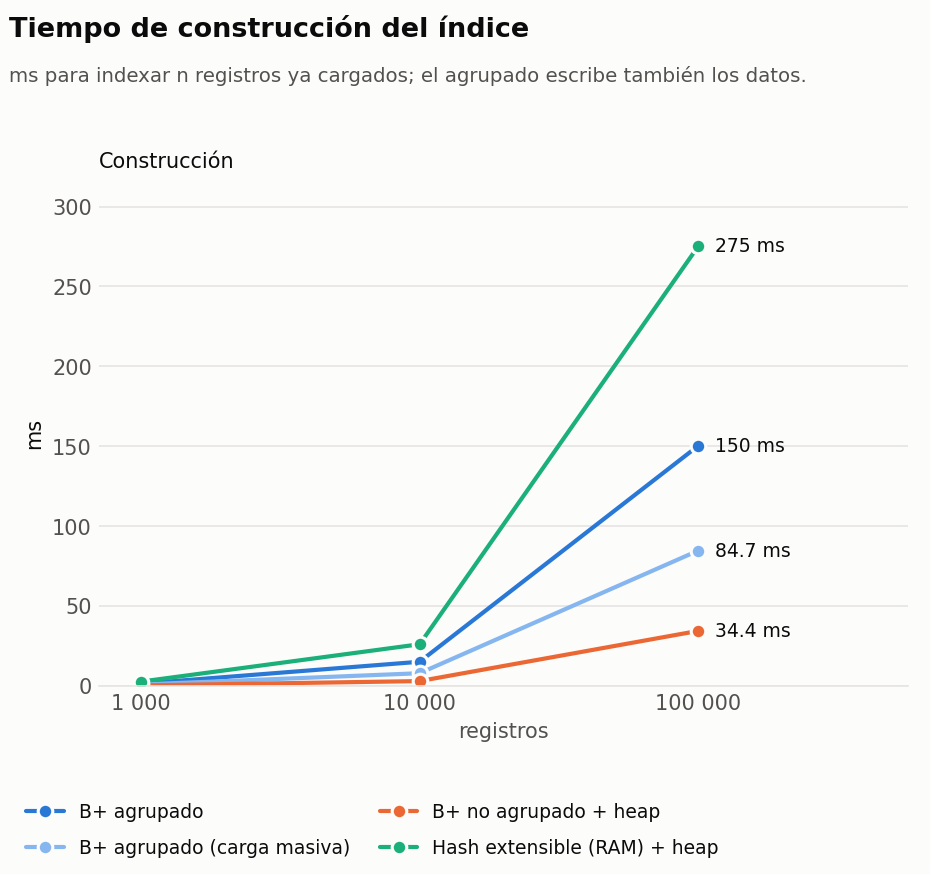
\includegraphics[width=0.7\textwidth]{img/01_construccion.png}
\caption{Tiempo de construcción del índice.}
\end{figure}

\begin{figure}[!htbp]
\centering
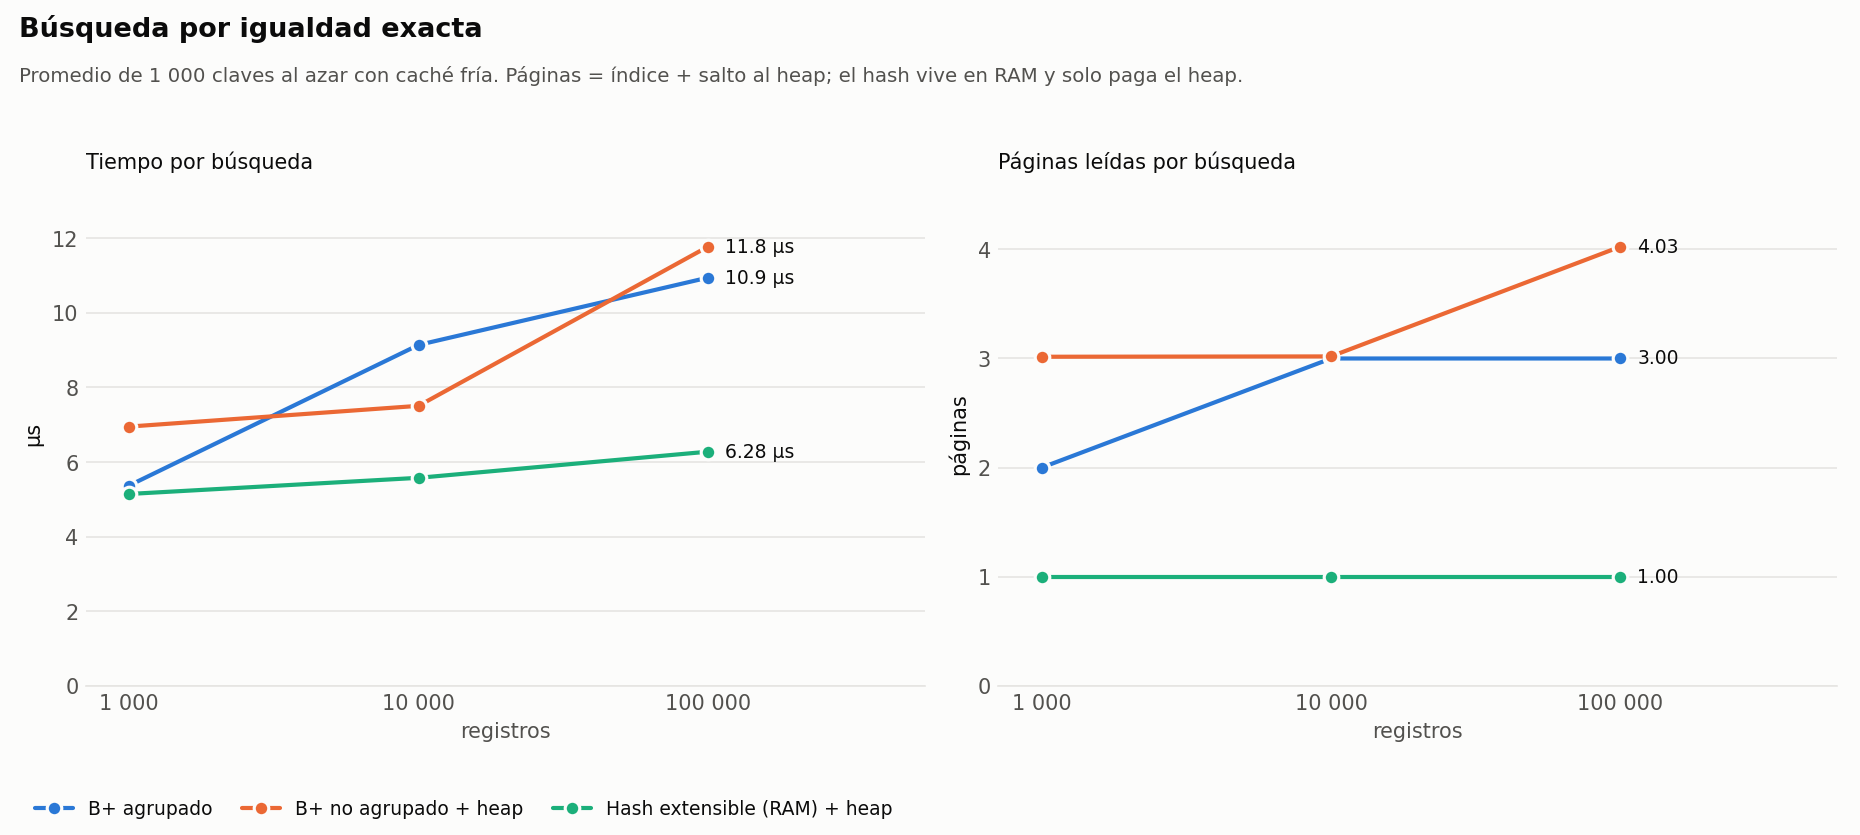
\includegraphics[width=\textwidth]{img/02_igualdad.png}
\caption{Búsqueda por igualdad: tiempo y páginas leídas.}
\end{figure}

\begin{figure}[!htbp]
\centering
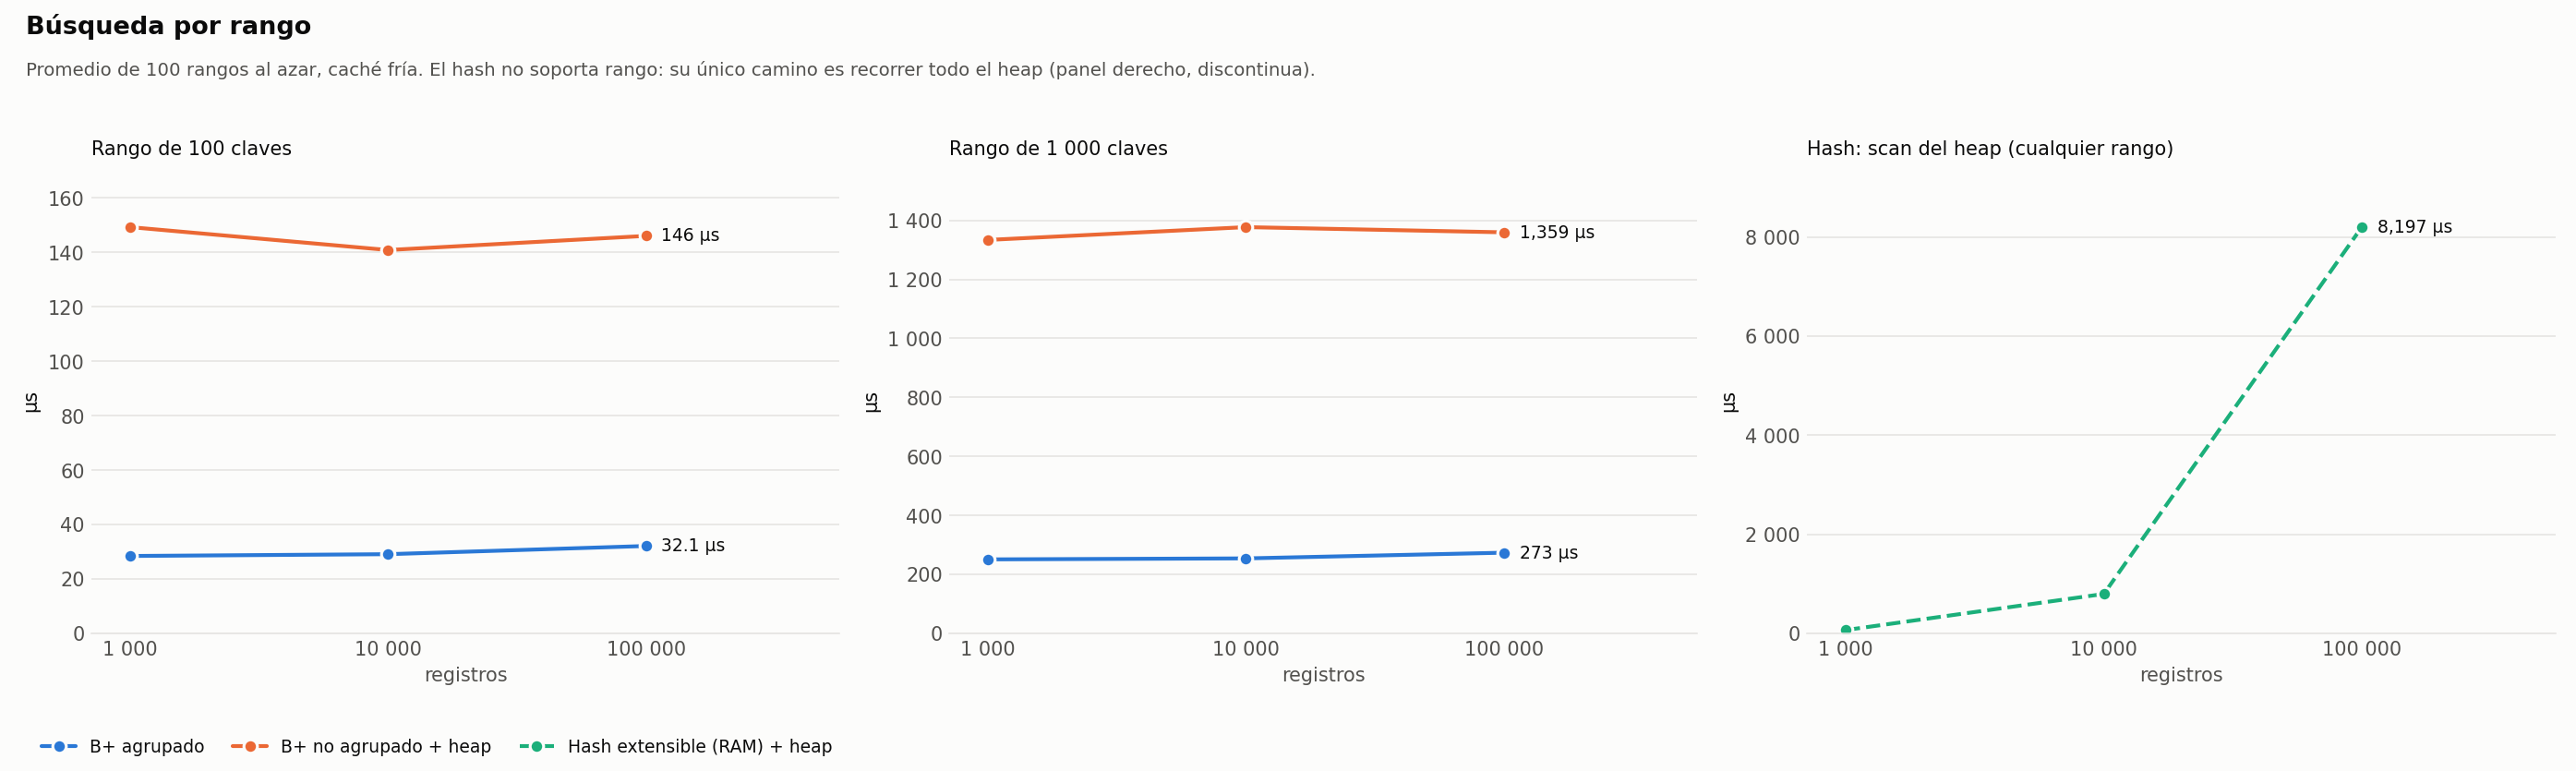
\includegraphics[width=\textwidth]{img/03_rango.png}
\caption{Búsqueda por rango de 100 y 1\,000 claves.}
\end{figure}

\begin{figure}[!htbp]
\centering
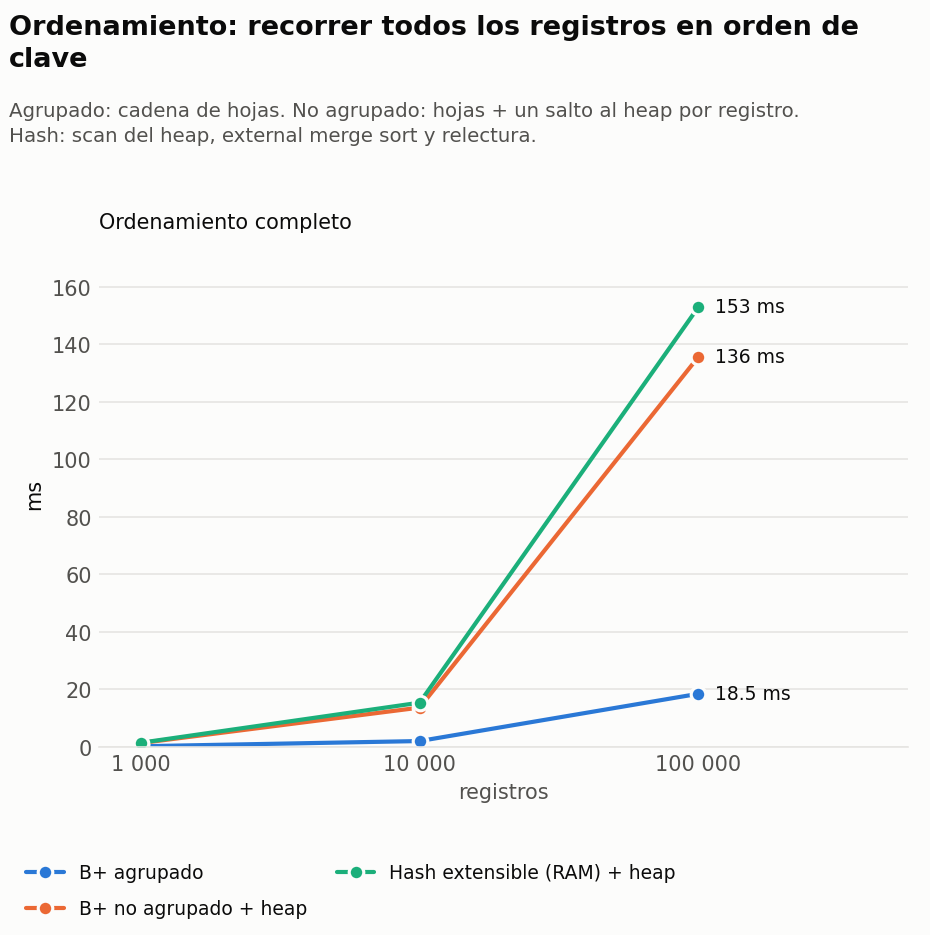
\includegraphics[width=0.7\textwidth]{img/04_ordenamiento.png}
\caption{Ordenamiento completo por clave.}
\end{figure}

\begin{figure}[!htbp]
\centering
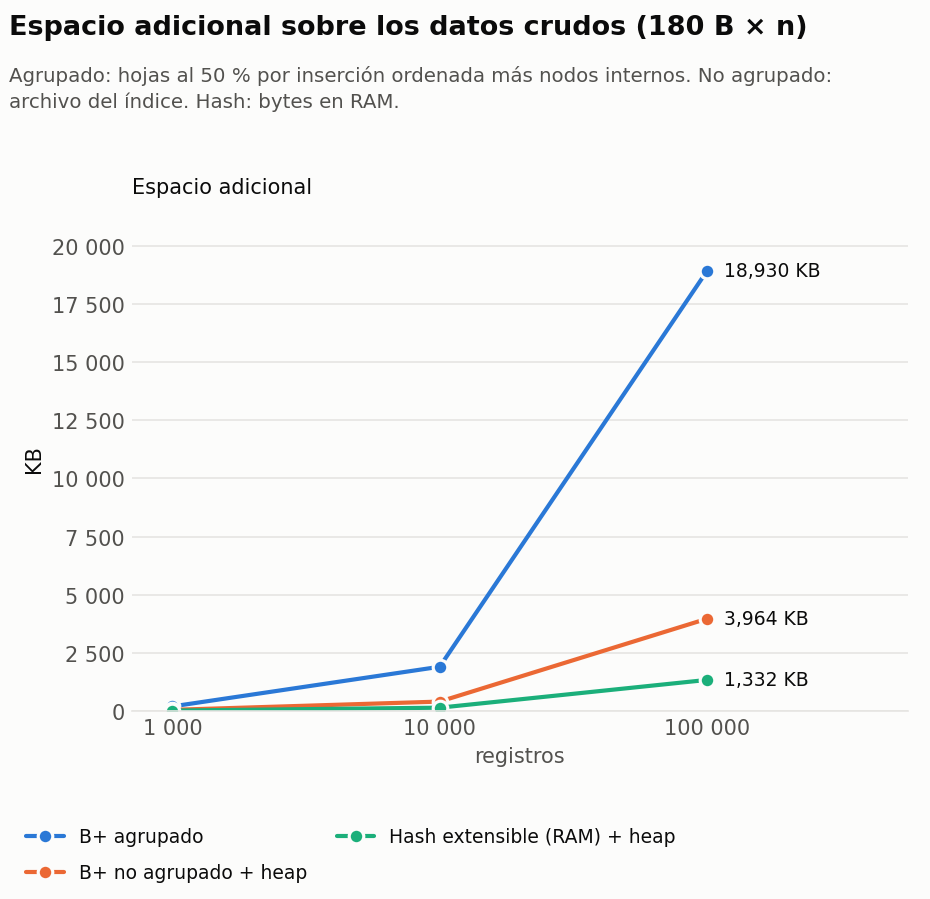
\includegraphics[width=0.7\textwidth]{img/05_espacio.png}
\caption{Espacio adicional sobre los datos.}
\end{figure}

\begin{figure}[!htbp]
\centering
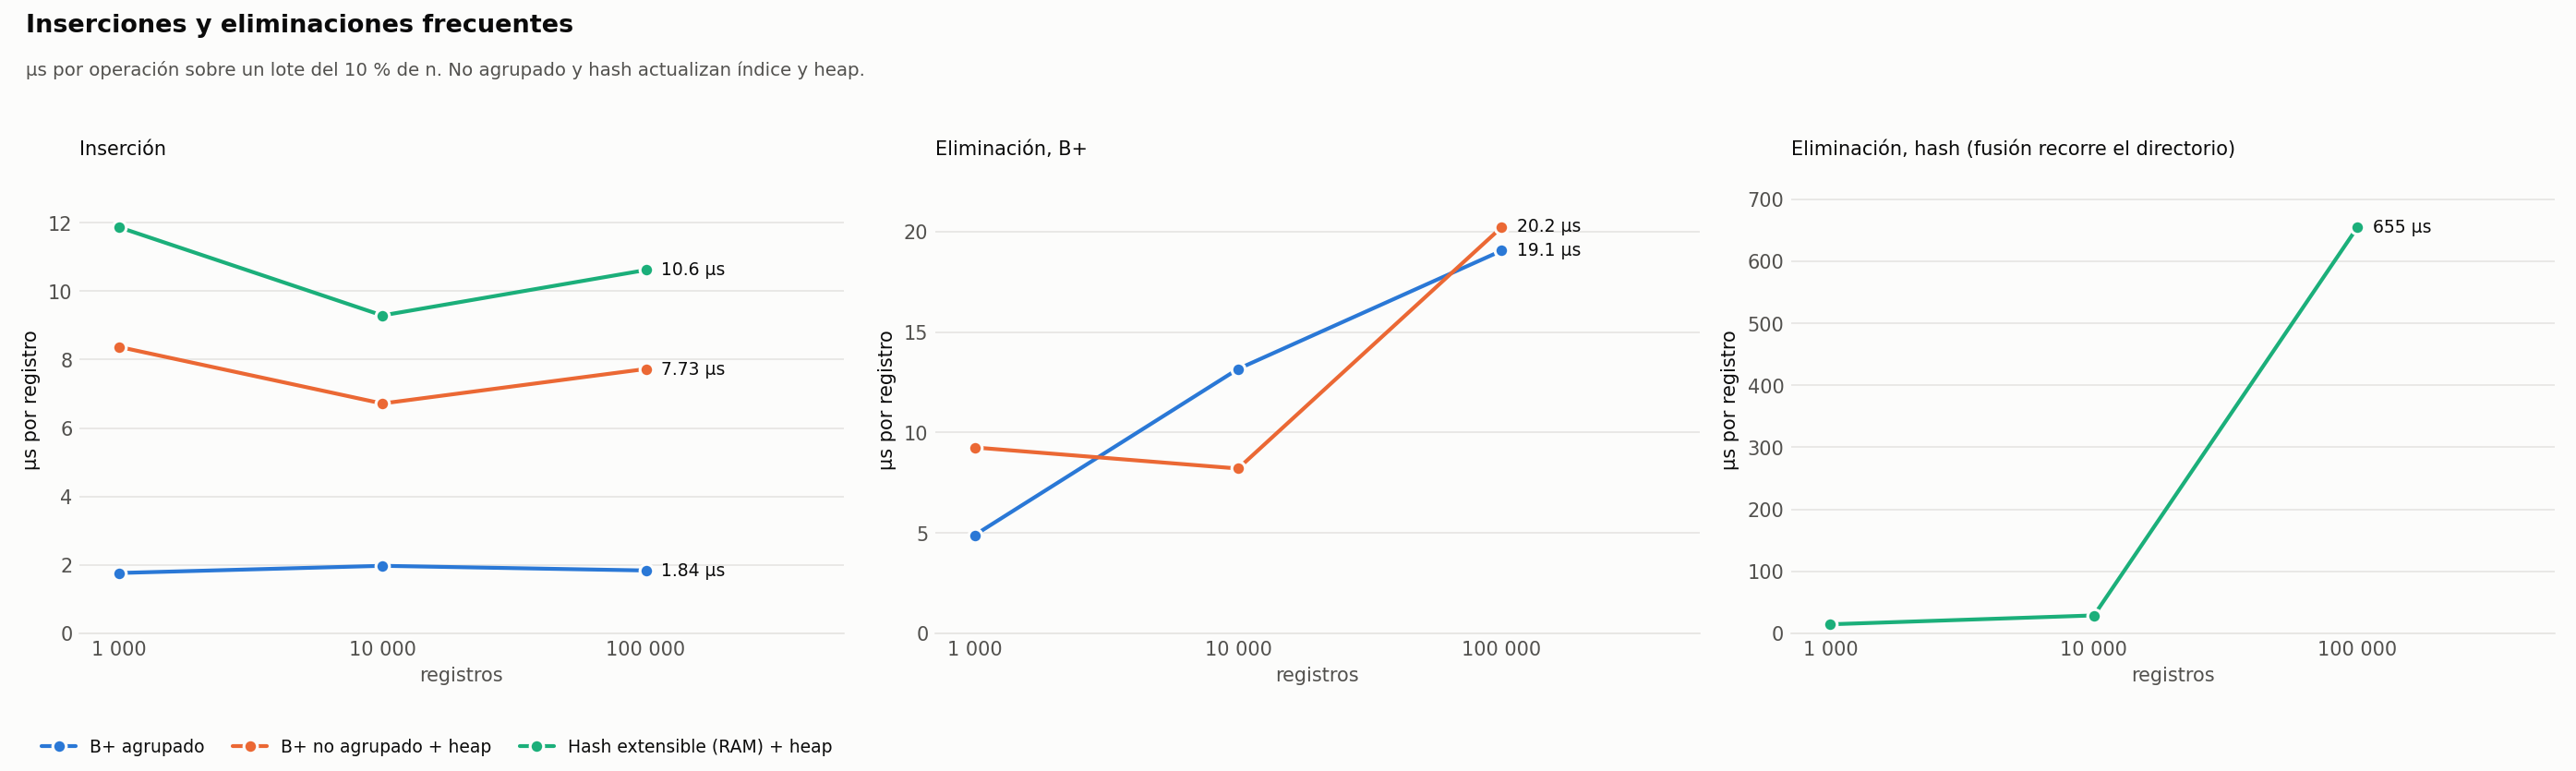
\includegraphics[width=\textwidth]{img/06_insercion_eliminacion.png}
\caption{Inserciones y eliminaciones frecuentes.}
\end{figure}

\begin{itemize}
  \item \emph{Igualdad.} Los tres responden entre 6 y 12 µs. Es la única operación donde el hash gana, y lo hace por poco.
  \item \emph{Rango.} Para 100 claves, el agrupado lee 12 páginas (hojas consecutivas) y el no agrupado 104, porque paga un salto al heap por cada fila. El hash no soporta rangos y debe recorrer todo el heap: 4\,546 páginas con 100\,000 filas.
  \item \emph{Ordenamiento.} El agrupado devuelve las 100\,000 filas ordenadas en 18 ms recorriendo sus hojas; el no agrupado tarda 136 ms y el hash 153 ms, porque además debe ordenar.
  \item \emph{Construcción.} En la gráfica el agrupado parece más lento (150 ms frente a 34 ms del no agrupado con 100\,000 filas), y esa fue una observación del primer avance. La diferencia está en lo que se mide: el agrupado escribe las filas completas, mientras que el tiempo del no agrupado no incluye cargar el heap (680 ms adicionales). Sumando datos e índice, el agrupado es unas cinco veces más rápido, y con carga masiva baja a 85 ms.
  \item \emph{Inserción.} El agrupado inserta en 1.8 µs porque mantiene una sola estructura; los otros dos escriben en el heap y en el índice, entre 8 y 11 µs.
\end{itemize}

\subsection{B+ agrupado frente a B+ no agrupado a través de SQL}

La misma comparación se repitió con el motor SQL completo, creando una tabla \texttt{USING BPLUS} y otra \texttt{USING HEAP} con índices secundarios, sobre 100\,000 filas:

\begin{table}[H]
\centering
\begin{tabular}{lrr}
\toprule
Operación & B+ agrupado & Heap + B+ no agrupado \\
\midrule
Construcción & 349 ms & 396 ms \\
Búsqueda puntual & 0.26 ms, 5 páginas & 5.6 ms, 4 páginas \\
Rango del 3\,\% & 9.0 ms, 237 páginas & 16.7 ms, 3\,033 páginas \\
Recorrido completo & 166 ms, 7\,698 páginas & 157 ms, 3\,709 páginas \\
Tamaño en disco & 31.6 MB & 15.2 MB \\
\bottomrule
\end{tabular}
\caption{B+ agrupado frente a heap con B+ no agrupado, 100\,000 filas.}
\end{table}

El agrupado gana en búsquedas y rangos porque la fila está en la hoja. Pierde un poco en los recorridos completos porque sus hojas guardan registros de tamaño fijo y ocupa el doble de páginas.

\subsection{Transacciones}
\label{sec:demo}

La demostración con hilos (\texttt{make demo-transacciones}) lanza 4 hilos que hacen 5 depósitos de 100 cada uno sobre la misma cuenta. Cada depósito lee el saldo, espera 5 ms y escribe el saldo nuevo. Se corre dos veces:

\begin{lstlisting}
sin transacciones:   esperado 2000, obtenido 500, depositos perdidos 15
con BEGIN/END y 2PL: esperado 2000, obtenido 2000, deadlocks detectados 31
\end{lstlisting}

Sin transacciones, cada sentencia es atómica, pero entre la lectura y la escritura otro hilo lee el mismo saldo y uno de los depósitos se pierde (\emph{lost update}). En las corridas realizadas se perdieron entre 13 y 15 de los 20 depósitos. Con \texttt{BEGIN ... END}, el lock compartido de la lectura se mantiene hasta escribir; cuando dos hilos leen y luego quieren escribir, se produce un deadlock que el gestor detecta, la víctima se deshace y reintenta, y el saldo final siempre es 2\,000. El número exacto de deadlocks varía entre corridas porque depende de cómo el sistema operativo reparte los hilos, pero la conclusión no cambia. Los eventos de locks se exportan a \texttt{datos/resultados/transacciones\_eventos.json} para que la interfaz pueda dibujarlos.

\subsection{Parte 2: R-Tree frente a búsqueda secuencial}

La prueba \texttt{rtree\_test} inserta 100\,000 puntos al azar alrededor de Lima (semilla 42) y compara el R-Tree con una búsqueda secuencial sobre los mismos puntos:

\begin{table}[H]
\centering
\begin{tabular}{lr}
\toprule
Medida & Valor \\
\midrule
Altura del árbol & 3 \\
Nodos & 872 \\
Tamaño en disco & 3\,492 KB \\
Nodos visitados, radio de 1 km & 14 de 872 \\
Nodos visitados, k = 10 & 8 de 872 \\
\bottomrule
\end{tabular}
\caption{R-Tree con 100\,000 puntos.}
\end{table}

Las 60 consultas de rango (radios de 1, 5 y 10 km con las dos métricas) y las 30 de k vecinos (k = 10, 50 y 100) devuelven exactamente lo mismo que la búsqueda secuencial. La diferencia está en lo que se lee: la búsqueda secuencial siempre recorre los 100\,000 puntos, mientras que el R-Tree resuelve un radio de 1 km leyendo 14 nodos y los 10 vecinos más cercanos leyendo 8.

\subsection{Parte 2: secuencial, R-Tree y GiST}

Para la sección 2.2.4 se midieron tres técnicas sobre los mismos puntos: la búsqueda secuencial y el R-Tree a través del motor SQL (\texttt{make bench-espacial}), y el índice GiST de PostgreSQL 18 sobre el tipo \texttt{point} nativo (\texttt{datos/resultados/gist\_bench.sql}). Los puntos se generan con el mismo generador congruencial en C++ y en SQL, y las sumas de coordenadas coinciden en los dos lados. Cada tiempo es el promedio de 100 consultas con la métrica euclidiana, que es la que calcula GiST sin PostGIS. En los 18 casos, las tres técnicas devuelven el mismo número de filas.

\begin{table}[H]
\centering
\small
\begin{tabular}{lrrrr}
\toprule
Consulta (100\,000 puntos) & Filas & Secuencial & R-Tree & GiST \\
\midrule
Rango de 1 km & 126 & 52,8 ms & 5,7 ms & 0,54 ms \\
Rango de 5 km & 2\,895 & 53,5 ms & 25,4 ms & 2,82 ms \\
Rango de 10 km & 10\,370 & 54,2 ms & 73,7 ms & 7,16 ms \\
k-NN, k = 10 & 10 & 342,6 ms & 5,0 ms & 0,19 ms \\
k-NN, k = 50 & 50 & 326,4 ms & 5,1 ms & 0,62 ms \\
k-NN, k = 100 & 100 & 409,5 ms & 5,7 ms & 0,56 ms \\
Construcción del índice & & & 5\,116 ms & 424 ms \\
Tamaño del índice & & & 3\,448 KB & 6\,528 KB \\
\bottomrule
\end{tabular}
\caption{Búsqueda secuencial, R-Tree del motor y GiST de PostgreSQL con 100\,000 puntos.}
\end{table}

\begin{figure}[!htbp]
\centering
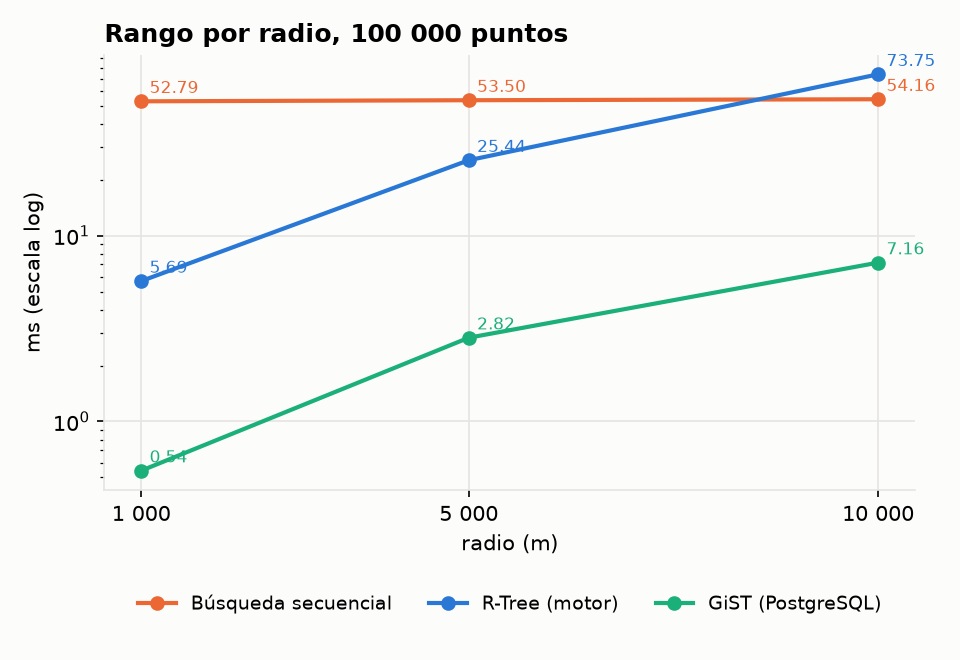
\includegraphics[width=0.75\textwidth]{img/espacial_rango.png}
\caption{Rango por radio con 100\,000 puntos (escala logarítmica).}
\end{figure}

\begin{figure}[!htbp]
\centering
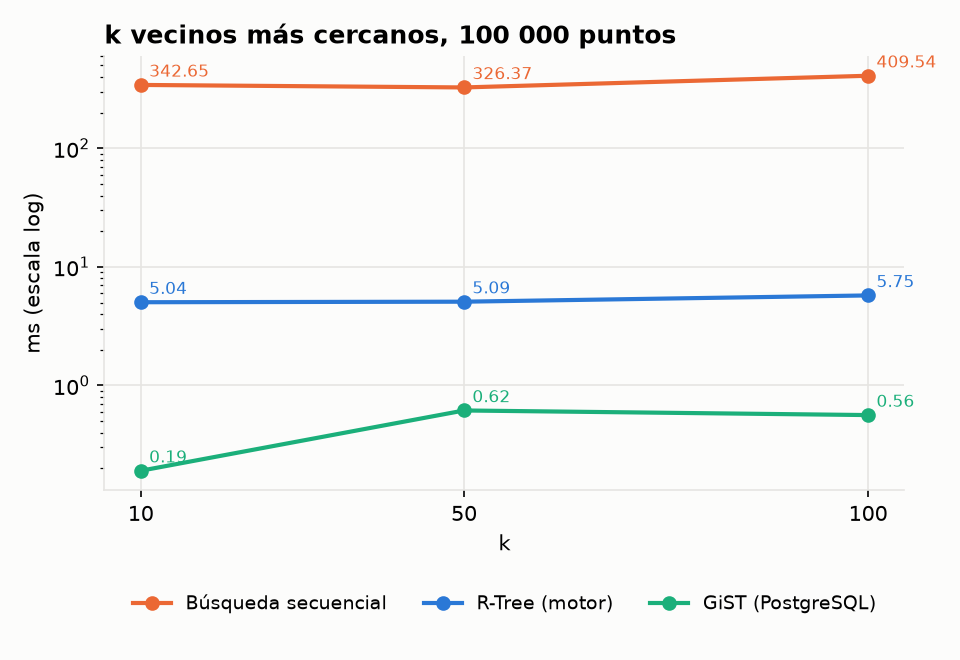
\includegraphics[width=0.75\textwidth]{img/espacial_knn.png}
\caption{k vecinos más cercanos con 100\,000 puntos (escala logarítmica).}
\end{figure}

La búsqueda secuencial cuesta lo mismo con cualquier radio, porque siempre lee las 491 páginas del heap. El R-Tree es unas 9 veces más rápido con un radio de 1 km, pero su costo crece con el número de filas encontradas, ya que por cada una lee una página del heap. Con 10 km la consulta devuelve el 10\,\% de la tabla y el R-Tree termina siendo más lento que el recorrido, el mismo efecto que se observó con el B+ no agrupado en rangos anchos. En k vecinos la diferencia es mucho mayor: la búsqueda secuencial calcula la distancia de todos los puntos y ordena la tabla completa, mientras que el R-Tree solo baja por los nodos más cercanos y es entre 64 y 71 veces más rápido, casi sin depender de k.

GiST resultó unas 10 veces más rápido que el R-Tree del motor en todas las consultas, aunque su índice ocupa casi el doble. Parte de esa diferencia no viene de la estructura: cada consulta del motor abre los archivos y lee el catálogo, mientras que PostgreSQL trabaja con la tabla ya en memoria compartida. Por eso la comparación más justa es la forma en que crece cada técnica, y en eso el R-Tree y GiST se comportan igual. La construcción del R-Tree es más lenta porque inserta punto por punto leyendo cada fila del heap. El detalle completo está en \texttt{docs/comparacion\_espacial/README.md}.

\subsection{Cuándo usar cada técnica}

\begin{table}[H]
\centering
\small
\begin{tabular}{p{3cm}p{5.2cm}p{5.8cm}}
\toprule
Técnica & Conviene cuando & Desventaja \\
\midrule
Heap File & hay muchas inserciones y recorridos completos & buscar por clave sin índice es un recorrido \\
Secuencial & se busca por clave o por rango y se inserta poco & inserciones lentas y reorganizaciones \\
B+ agrupado & se consulta por rango o se lista ordenado por la clave primaria & solo uno por tabla; ocupa más páginas \\
B+ no agrupado & se necesita un índice secundario con repetidos, por igualdad o rango & una lectura del heap por cada fila devuelta \\
Hash extensible & solo hay búsquedas por igualdad & no sirve para rangos ni para ordenar \\
R-Tree & se busca por distancia a un punto o dentro de un polígono, con pocas filas en el resultado & radios que devuelven gran parte de la tabla \\
\bottomrule
\end{tabular}
\caption{Resumen de ventajas y desventajas.}
\end{table}

%-------------------------------------------------------------------------------
\section{Conclusiones y límites conocidos}
\label{sec:pendiente}

El proyecto permitió comprobar en la práctica varias ideas que en clase se ven de forma teórica. La más clara es que el número de páginas leídas explica casi todas las diferencias de rendimiento: el secuencial gana en búsquedas porque lee 35 páginas en lugar de 1\,598, y el B+ agrupado gana en rangos porque sus filas están contiguas. También quedó claro que medir bien es parte del trabajo, porque dos de las observaciones del primer avance se explicaban por qué se estaba midiendo y no por un error en las estructuras.

La Parte 1 está completa, con dos límites. El motor no implementa \texttt{JOIN} aunque los algoritmos de hash join e index nested loop join ya están escritos en \texttt{external\_algorithms.h}; falta conectarlos al parser y al ejecutor. Los locks son a nivel de tabla, lo que simplifica el gestor pero reduce la concurrencia frente a locks por registro.

De la Parte 2 están terminados el tipo \texttt{POINT}, las dos métricas de distancia, la extensión SQL, el índice R-Tree con sus tres consultas (radio, k vecinos y polígono), el panel de mapa en la interfaz y la comparación con GiST. La comparación dejó una lección parecida a la de la Parte 1: un índice ayuda mucho cuando la consulta devuelve pocas filas, como en k vecinos o en radios chicos, pero deja de convenir cuando devuelve una parte grande de la tabla, porque cada fila cuesta una página del heap. También mostró que una implementación propia sigue la misma forma que GiST, aunque PostgreSQL es unas 10 veces más rápido por todo lo que optimiza fuera de la estructura. El repositorio ya incluye \texttt{postgis\_bench.sql}, que repite la comparación con PostGIS sobre \texttt{geography} y distancia geodésica; como trabajo futuro queda ejecutarlo y comparar esos tiempos con la métrica haversine del motor.

\section*{Referencias}
\begin{enumerate}
  \item Garcia-Molina, H., Ullman, J. D. y Widom, J. \emph{Database Systems: The Complete Book}. Pearson, 2.ª edición, 2008.
  \item Ramakrishnan, R. y Gehrke, J. \emph{Database Management Systems}. McGraw-Hill, 3.ª edición, 2003.
  \item Fagin, R., Nievergelt, J., Pippenger, N. y Strong, H. R. Extendible hashing: a fast access method for dynamic files. \emph{ACM Transactions on Database Systems}, 4(3), 1979.
  \item Guttman, A. R-trees: a dynamic index structure for spatial searching. \emph{Proceedings of ACM SIGMOD}, 1984.
  \item PostgreSQL Global Development Group. Documentación de \texttt{EXPLAIN}.\\ \url{https://www.postgresql.org/docs/current/sql-explain.html}
\end{enumerate}

\end{document}
